% ============================================================================
% QCD: quark-antiquark annihilation into two gluons, s-channel diagram (three-gluon vertex), lowest order
%        q_i(p,s) + qbar_j(k,r)  ->  g*(q)  ->  g^b(k1,l1) + g^c(k2,l2)
% This is the diagram with NO QED analogue: the off-shell gluon splits through the non-abelian three-gluon vertex.
% (The t- and u-channel quark-exchange diagrams of qqbar -> gg are the ones that resemble e+e- -> gamma gamma.)
% First pair q, qbar blue; internal gluon black coil; outgoing gluons red coils.
%
% Conventions as in qcd_rules.tex (Feynman gauge, D_mu = d_mu - i g A^a_mu t^a):
%   quark-gluon vertex     i g gamma^mu t^a_{ji}   (j = outgoing colour, i = incoming colour along the fermion line)
%   gluon propagator       -i g_{mu nu} delta^{ad} / (q^2 + i eps),   q = p + k = k1 + k2,   q^2 = s
%   three-gluon vertex     g f^{dbc} [ g^{nu rho}(q+k1)^sigma + g^{rho sigma}(k2-k1)^nu - g^{sigma nu}(q+k2)^rho ]
%                          (all momenta incoming: (nu,d,q), (rho,b,-k1), (sigma,c,-k2))
%   amplitude   iM_s = [ vbar_j(k) (i g gamma^mu t^a_{ji}) u_i(p) ] (-i g_{mu nu} delta^{ad}/q^2)
%                      * g f^{dbc} [ ... ]^{nu rho sigma} eps*_rho(k1) eps*_sigma(k2)
% Fermion arrows: incoming quark towards the vertex, incoming antiquark away from the vertex (against its momentum).
% Colour indices: quarks i,j = 1..3 ; gluons a,b,c,d = 1..8.
% Page = PowerPoint widescreen (13.333in x 7.5in).  Compile with pdflatex or lualatex.
% ============================================================================
\documentclass[10pt]{article}
\usepackage{lmodern}
\usepackage[T1]{fontenc}
\usepackage{amsmath,amssymb}
\usepackage{xcolor}
\usepackage{graphicx}
\usepackage{tikz}
\usetikzlibrary{decorations.markings,decorations.pathmorphing,arrows.meta,positioning,calc}
\usepackage[paperwidth=338.67mm,paperheight=190.5mm,
            left=5mm,right=5mm,top=3mm,bottom=3mm]{geometry}
\pagestyle{empty}
\setlength{\parindent}{0pt}

\definecolor{qcol}{HTML}{1F4E9C}   % quark pair q, qbar (same blue as the electron / the QCD rules page)
\definecolor{rcol}{HTML}{C0392B}   % outgoing gluons (same red as the muon / the second quark before)

\tikzset{
  bf/.style={line width=2.4pt,                               % quark line with arrow
    decoration={markings,
      mark=at position 0.55 with {\arrow{Stealth[length=4.4mm,width=3.6mm]}}},
    postaction={decorate}},
  bmom/.style={-{Stealth[length=2.8mm,width=2.3mm]},line width=1pt,color=black!70},
  qlab/.style={font=\fontsize{30}{34}\selectfont,text=qcol,inner sep=2pt},
  rlab/.style={font=\fontsize{30}{34}\selectfont,text=rcol,inner sep=2pt},
  plab/.style={font=\fontsize{28}{32}\selectfont,inner sep=2pt},
  qvbox/.style={font=\fontsize{27}{31}\selectfont,text=qcol,draw=qcol,fill=qcol!8,
                line width=1.2pt,rounded corners=4pt,inner sep=7pt},
  gvbox/.style={font=\fontsize{19}{22}\selectfont,text=rcol,draw=rcol,fill=rcol!8,
                line width=1.2pt,rounded corners=4pt,inner sep=6pt},
  pbox/.style={font=\fontsize{30}{34}\selectfont,draw=black!60,fill=black!4,
               line width=1.2pt,rounded corners=4pt,inner sep=8pt},
  gl/.style={line width=1.8pt,decorate,
             decoration={coil,aspect=0.5,segment length=0.575cm,amplitude=2.1mm}},
}

\begin{document}
\vspace*{\fill}
\centering
\scalebox{1.1}{%
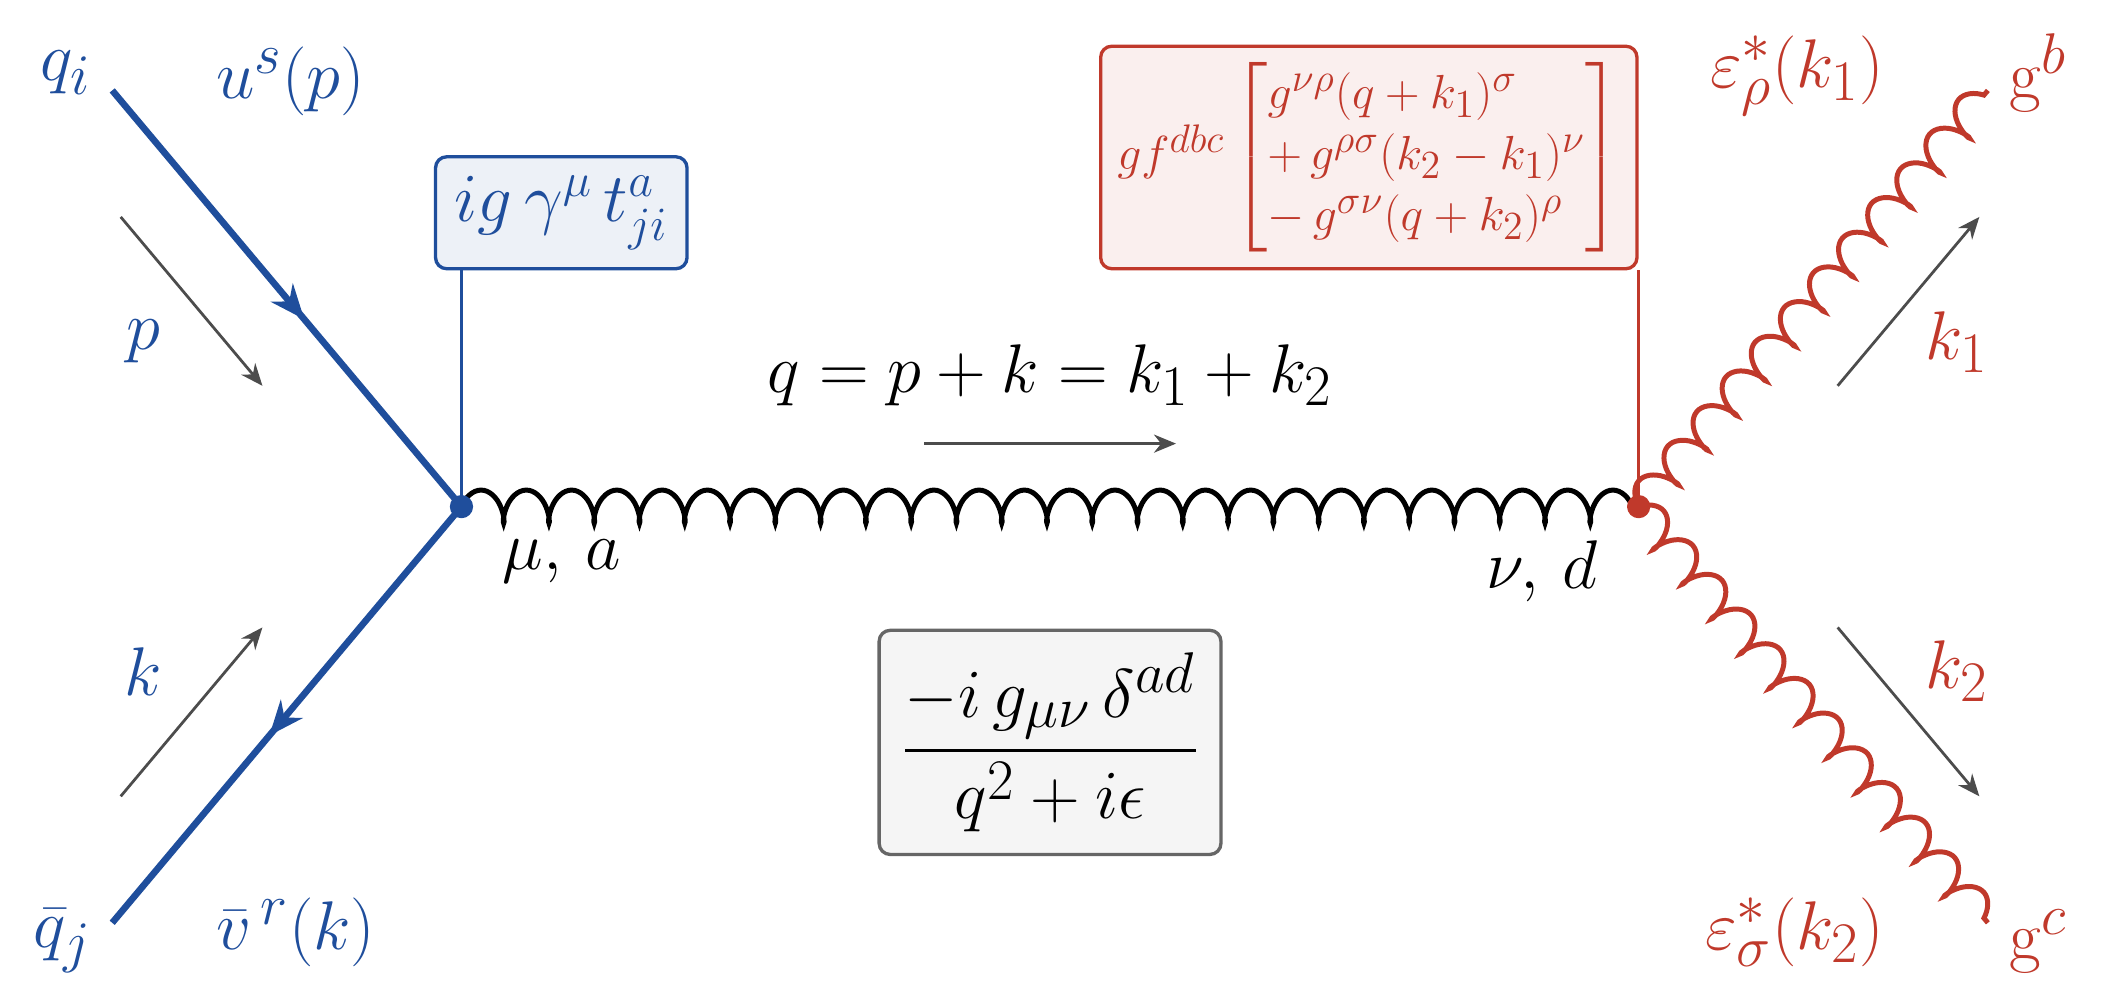
\begin{tikzpicture}[x=1cm,y=1cm]
  % vertices on the horizontal axis; legs leave at +-50 degrees from the vertical
  \coordinate (V1) at (-7.475,0);                            % annihilation vertex   q qbar -> g*
  \coordinate (V2) at ( 7.475,0);                            % three-gluon vertex    g* -> g g
  \coordinate (E1) at ($(V1)+(130:6.9)$);                    % q     in   (upper left)
  \coordinate (E2) at ($(V1)+(230:6.9)$);                    % qbar  in   (lower left)
  \coordinate (E3) at ($(V2)+(50:6.9)$);                     % g(k1) out  (upper right)
  \coordinate (E4) at ($(V2)+(310:6.9)$);                    % g(k2) out  (lower right)
  % coil segment length 0.575 cm everywhere: internal gluon = 26 coils (14.95 cm), outgoing gluons = 12 coils (6.9 cm)

  % ----------------------------------------------------------- quark lines (arrow = fermion flow)
  \draw[bf,color=qcol] (E1) -- (V1);                         % incoming quark q:      arrow towards the vertex
  \draw[bf,color=qcol] (V1) -- (E2);                         % incoming antiquark:    arrow away from the vertex

  % ----------------------------------------------------------- gluons (black coils)
  \draw[gl] (V1) -- (V2);                                    % internal s-channel gluon
  \draw[gl,color=rcol] (V2) -- (E3);                         % outgoing gluon 1 (red)
  \draw[gl,color=rcol] (V2) -- (E4);                         % outgoing gluon 2 (red)

  % ----------------------------------------------------------- vertices (dots + boxed vertex factors)
  \fill[qcol] (V1) circle (4.2pt);
  \fill[rcol] (V2) circle (4.2pt);
  \draw[qcol,line width=1.2pt] (V1) -- ($(V1)+(0,3.0)$);
  \draw[rcol,line width=1.2pt] (V2) -- ($(V2)+(0,3.0)$);
  \node[qvbox,anchor=south west,xshift=-3.5mm] at ($(V1)+(0,3.0)$) {$i g\,\gamma^{\mu}\,t^{a}_{ji}$};
  \node[gvbox,anchor=south east]               at ($(V2)+(0,3.0)$)
       {$g f^{dbc}\left[\begin{array}{@{}l@{}}
          g^{\nu\rho}(q+k_1)^{\sigma}\\
          +\,g^{\rho\sigma}(k_2-k_1)^{\nu}\\
          -\,g^{\sigma\nu}(q+k_2)^{\rho}
        \end{array}\right]$};

  % ----------------------------------------------------------- particle names and colour indices at the line ends
  \node[qlab,anchor=east] at ($(E1)+(130:0.3)$) {$q_{i}$};
  \node[qlab,anchor=east] at ($(E2)+(230:0.3)$) {$\bar q_{j}$};
  \node[rlab,anchor=west] at ($(E3)+(50:0.3)$)  {$\mathrm{g}^{b}$};
  \node[rlab,anchor=west] at ($(E4)+(310:0.3)$) {$\mathrm{g}^{c}$};

  % ----------------------------------------------------------- external wavefunctions (outside the lines)
  \node[qlab,anchor=south west] at ($(V1)+(130:5.8)+(40:0.7)$)  {$u^{s}(p)$};
  \node[qlab,anchor=north west] at ($(V1)+(230:5.8)+(320:0.7)$) {$\bar v^{\,r}(k)$};
  \node[rlab,anchor=south east] at ($(V2)+(50:5.8)+(140:0.7)$)  {$\varepsilon^{*}_{\rho}(k_1)$};
  \node[rlab,anchor=north east] at ($(V2)+(310:5.8)+(220:0.7)$) {$\varepsilon^{*}_{\sigma}(k_2)$};

  % ----------------------------------------------------------- momenta (inside the wedges)
  \draw[bmom] ($(V1)+(130:5.6)+(220:0.95)$) -- ($(V1)+(130:2.8)+(220:0.95)$);
  \node[plab,text=qcol] at ($(V1)+(130:4.2)+(220:1.75)$) {$p$};
  \draw[bmom] ($(V1)+(230:5.6)+(140:0.95)$) -- ($(V1)+(230:2.8)+(140:0.95)$);
  \node[plab,text=qcol] at ($(V1)+(230:4.2)+(140:1.75)$) {$k$};
  \draw[bmom] ($(V2)+(50:2.8)+(320:0.95)$) -- ($(V2)+(50:5.6)+(320:0.95)$);
  \node[plab,text=rcol] at ($(V2)+(50:4.2)+(320:1.75)$) {$k_1$};
  \draw[bmom] ($(V2)+(310:2.8)+(40:0.95)$) -- ($(V2)+(310:5.6)+(40:0.95)$);
  \node[plab,text=rcol] at ($(V2)+(310:4.2)+(40:1.75)$) {$k_2$};

  % ----------------------------------------------------------- internal gluon: indices, momentum, propagator
  \node[plab,anchor=north west] at ($(V1)+(0.45,-0.35)$) {$\mu,\,a$};
  \node[plab,anchor=north east] at ($(V2)+(-0.45,-0.35)$) {$\nu,\,d$};
  \draw[bmom] (-1.6,0.8) -- (1.6,0.8);
  \node[plab,anchor=south] at (0,1.2) {$q=p+k=k_1+k_2$};
  \node[pbox,anchor=north] at (0,-1.55) {$\displaystyle\frac{-i\,g_{\mu\nu}\,\delta^{ad}}{q^{2}+i\epsilon}$};
\end{tikzpicture}}
\vfill
\end{document}
